%課題研究レジュメテンプレート ver. 1.0

\documentclass[uplatex]{jsarticle}
\usepackage[top=20mm,bottom=20mm,left=20mm,right=20mm]{geometry}
\usepackage[T1]{fontenc}
\usepackage{txfonts}
\usepackage{wrapfig}
\usepackage[expert,deluxe]{otf}
\usepackage[dvipdfmx,hiresbb]{graphicx}

\makeatletter
  \renewcommand{\section}{%
    \if@slide\clearpage\fi
    \@startsection{section}{1}{\z@}%
    {\Cvs \@plus.5\Cdp \@minus.2\Cdp}% 前アキ
    {.5\Cvs \@plus.3\Cdp}% 後アキ
    %{\normalfont\Large\headfont\raggedright}}
    {\normalfont\raggedright}}

  \renewcommand{\subsection}{\@startsection{subsection}{2}{\z@}%
    {\Cvs \@plus.5\Cdp \@minus.2\Cdp}% 前アキ
    {.5\Cvs \@plus.3\Cdp}% 後アキ
    %{\normalfont\large\headfont}}
    {\normalfont}}

  \renewcommand{\subsubsection}{\@startsection{subsubsection}{3}{\z@}%
    {\Cvs \@plus.5\Cdp \@minus.2\Cdp}%
    {\z@}%
    %{\normalfont\normalsize\headfont}}
    {\normalfont}}
\makeatother
%ここから上を編集する必要はない.





\title{\vspace{-14mm}プログラミング学習を目的とするゲームサービスの実態調査}
\author{PMコース 矢吹研究室 1242034 小池 克人}
\date{}%日付を入れる必要はない.
\pagestyle{empty}%ページ番号は振らない.
\begin{document}
\maketitle





\section{研究の背景}

2013年6月5日に「アベノミクス」の「3本目の矢」として発表された成長戦略の素案の中にプログラミング教育が盛り込まれ\cite{koike001},プログラミングに対しての関心が高まっている.

ソフトウェア開発のプロジェクトにおいて個人がプログラミングを理解していることは重要である.その中でプログラミングを覚えていない人に理解してもらうのは急務である.プログラミングを学ぶスクールやプログラミング教室などが開催されているがそれに参加するには参加費と会場までの移動という負担が掛かるため,長続きするとは限らない.そこで本研究ではモチベーションを高める効果を持つゲーミフィケーションに着目した.

ゲーミフィケーションとは,理屈抜きに人を夢中にさせるゲームづくりのノウハウをゲーム以外の分野に応用して楽しみながら自ら進んで取り組む仕掛けをつくり出すことである\cite{koike002}.このゲーミフィケーションを成立させるためには4つの条件を満たす必要がある.それは何をするか明確になっていること,自分が今どういう状況なのかすぐにわかること,アクションに対してすぐに反応があること,ゴールしたり達成すると感動や御褒美をもらえるという条件である.この条件が様々な取り組みをゲーム化する最低条件である.

このゲーミフィングという手法に基づきプログラミング学習をゲームで実践した場合,ゲームでプログラミング習得の初期学習を効果的にできるのかを調査する.






\section{研究の目的}


\begin{itemize}
\item ゲーミフィケーションに着目し,プログラミング習得の初期学習を効果的にゲームで勉強できるのかを学生を対象に調査する.
\item 調査したゲームが実際にプログラミングの講義で使うことができるのかを計測する.

\end{itemize}





\section{プロジェクトマネジメントとの関連}

本研究はソフトウェア開発プロジェクトにおける各個人のプログラミングスキルの向上のためにゲーミフィケーションという手法を用いて初期プログラミング習得時に効率のよい手法を研究する.これは,人的資源マネジメントに関連づくと考えられる.








\section{研究の方法}

以下の順に研究を進める.

①フリーゲームの選別.

②ゲームの実施,データの収集.

③データマイニングの実施.


















\section{現在の進捗状況}

研究方法の②で集めたデータは,日本語対応しているか,ジャンル,難易度,対応言語数,登録が必要か,対応言語のデータを集めた.結果は,図1である.

ゲームのジャンルは,RPG,パズル,シミュレーション,クイズの4種類となった.難易度は,自分でゲームを実践して感じた難易度である.そして,学べる言語が一番多いのは,CodinGameというゲームで20個という結果になった.

この集めたデータを,統計処理ソフトウェアであるRを使ってマイニングし,自己組織化マップを作成し,分析を行なった.
この図を見ると左上が選択式のゲーム,左下がコードを入力するゲーム,右上が難易度が高いゲームに分類できる.





\makeatletter
\def\setcaption#1{\def\@captype{#1}}
\makeatother

\begin{center}


\begin{minipage}{8cm}
  \setcaption{table}
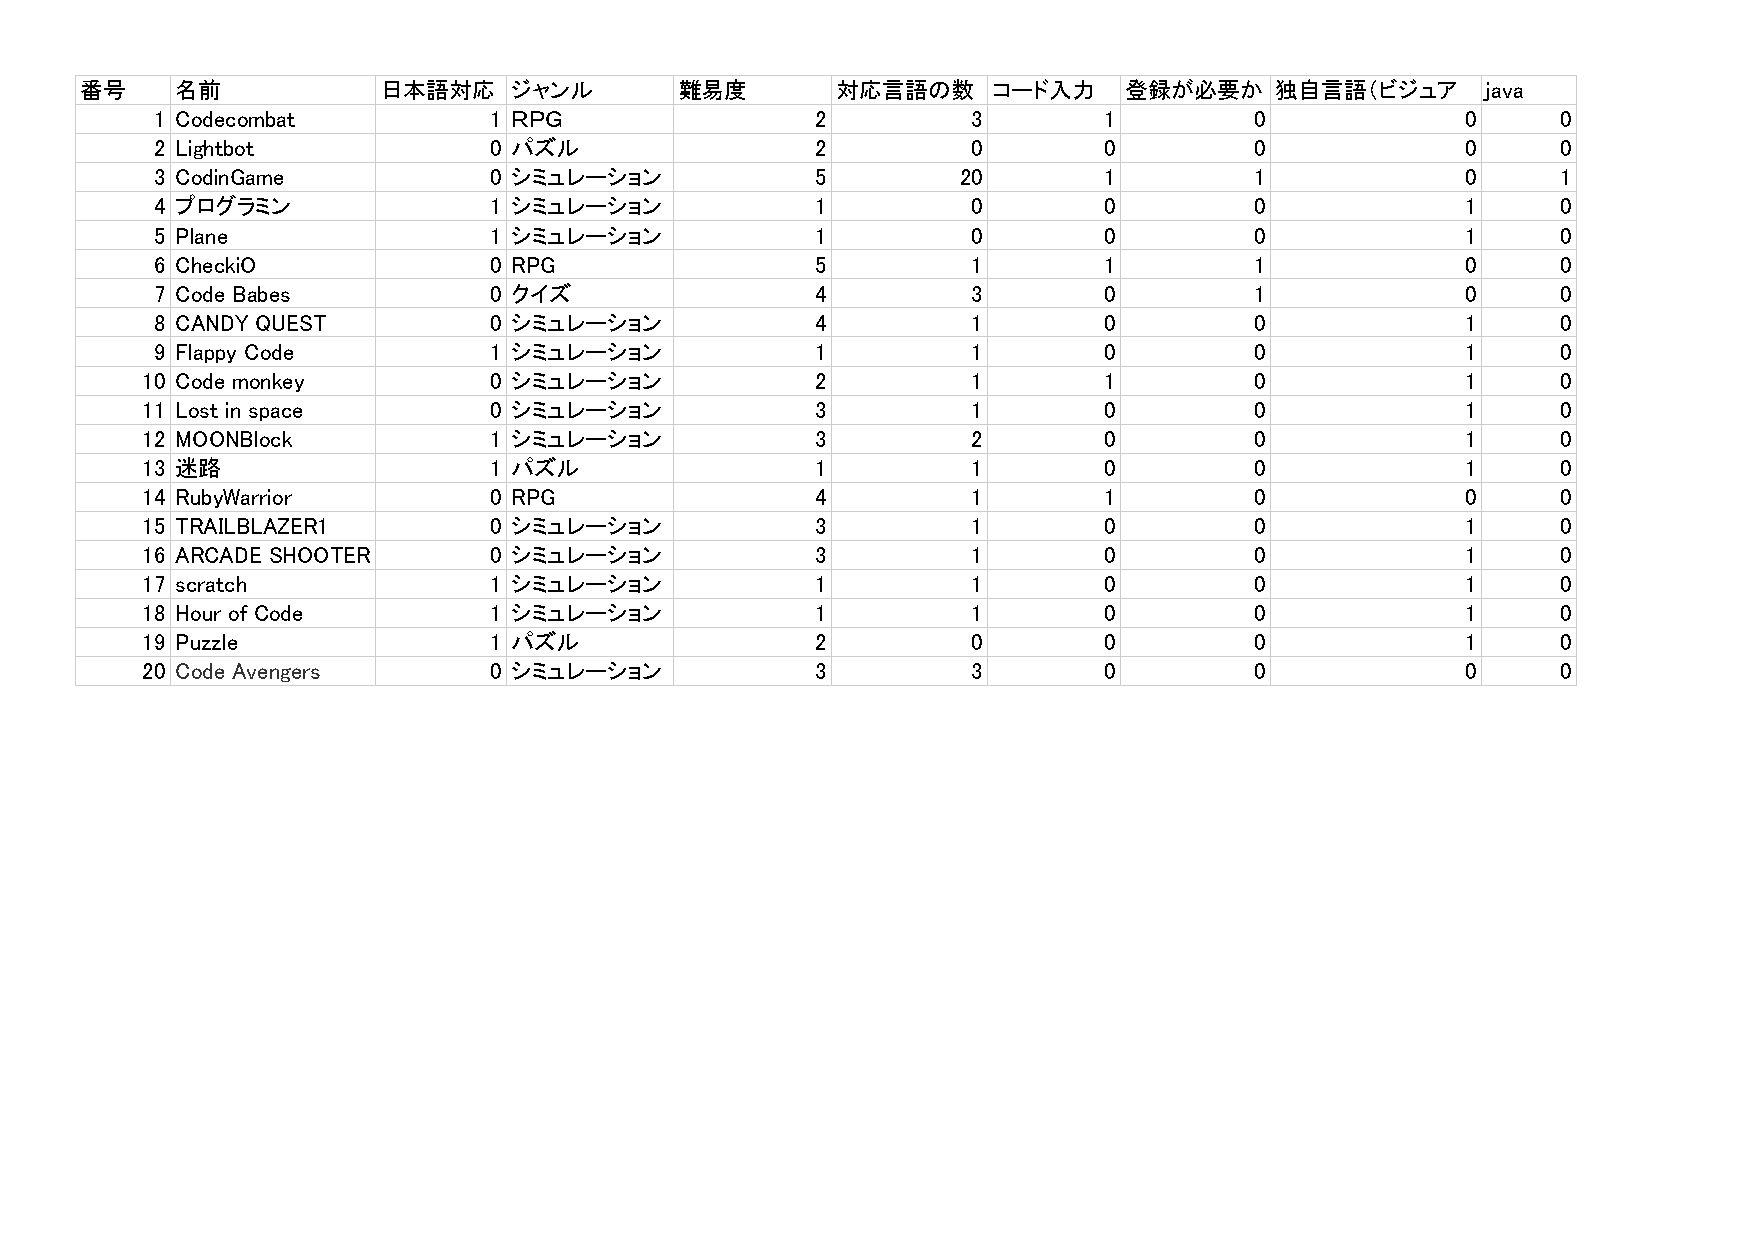
\includegraphics[width=8cm,clip]{gazou.pdf}
 \caption{集計データ}\label{サンプル図} 
\end{minipage} 
\begin{minipage}{10cm}
  \setcaption{figure}
\caption{自己組織化マップ}\label{サンプル図}
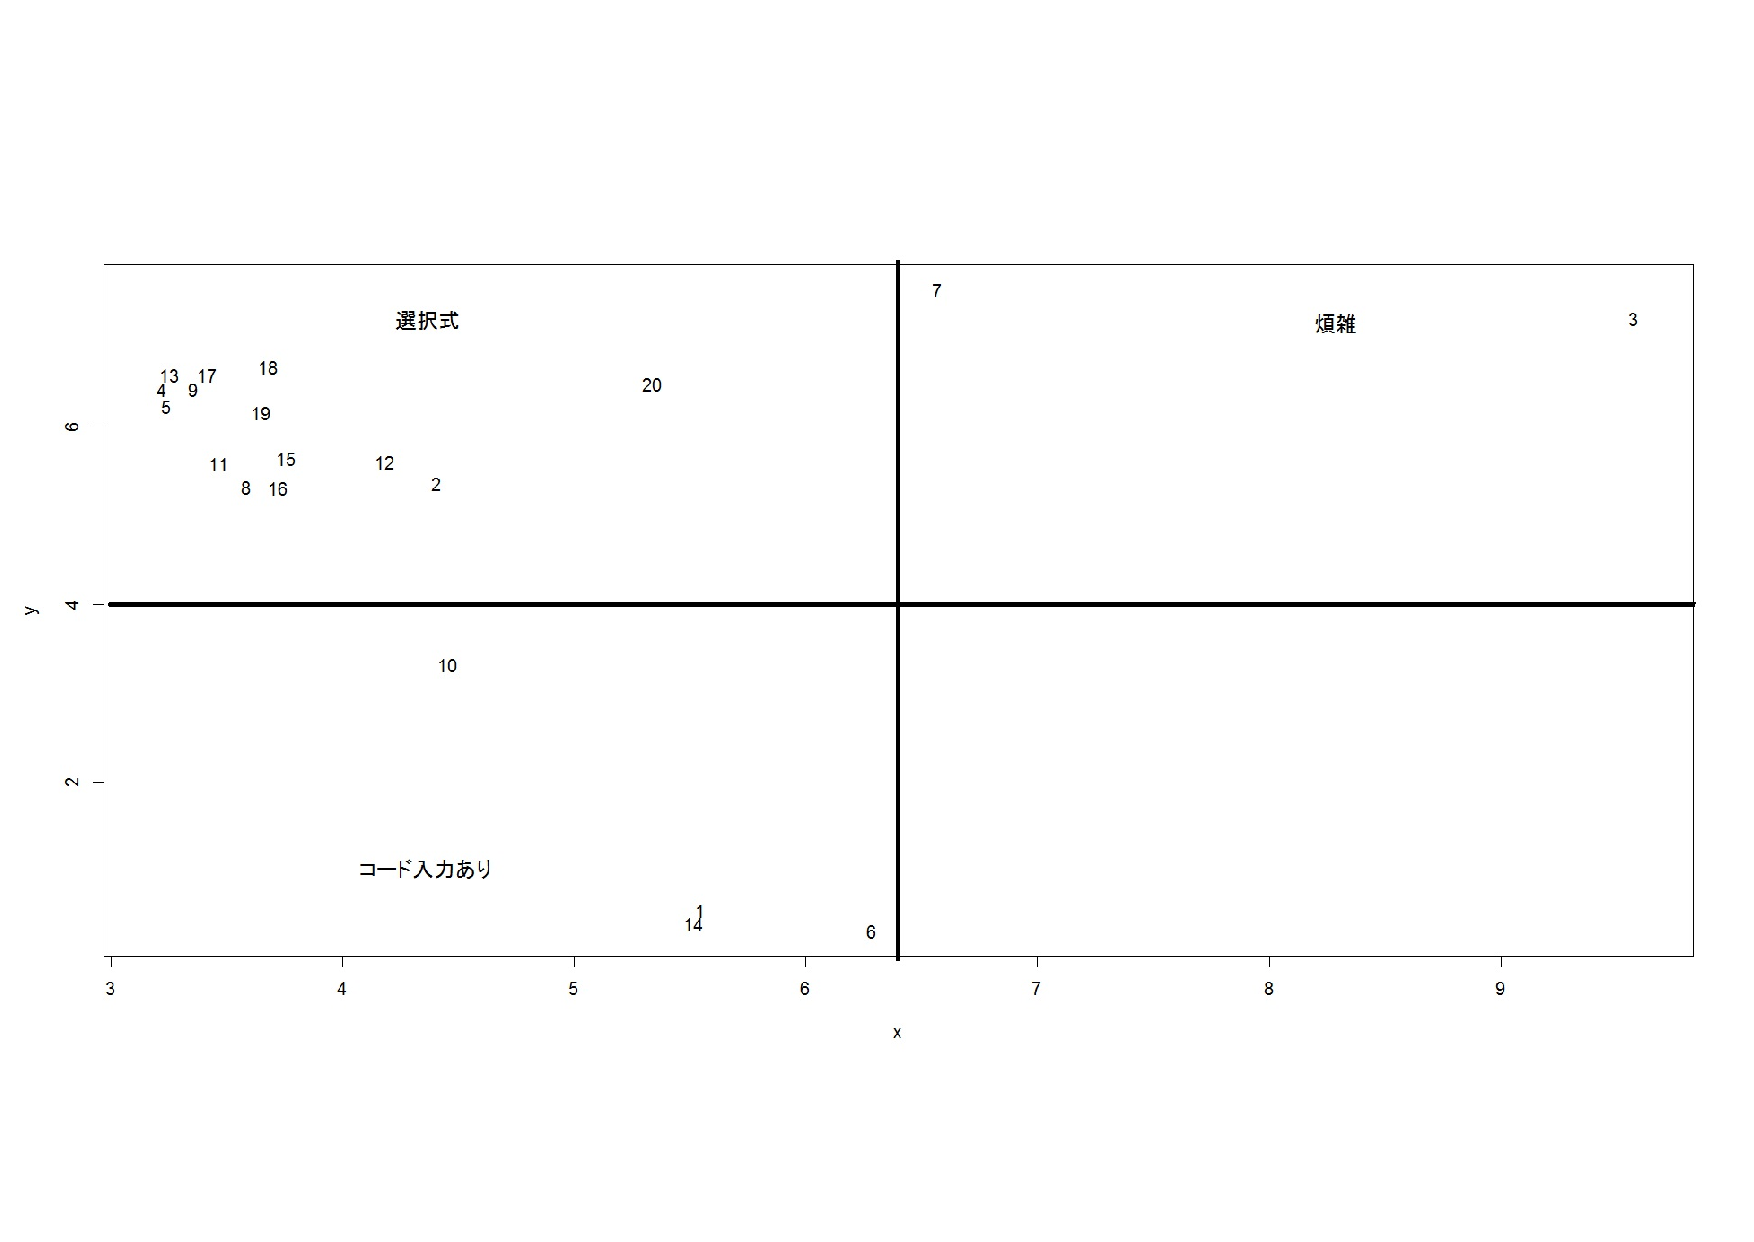
\includegraphics[width=10cm,clip]{figure.pdf}
\end{minipage}
\end{center}



\section{今後の計画}

以下のように研究を進める計画である.

\begin{enumerate}
\item 千葉工業大学のプログラミングの講義を調査する.
\item ゲームをPM実験の前の学生に行なわせ,調査する.
\end{enumerate}





\bibliographystyle{junsrt}
\bibliography{biblio}%「biblio.bib」というファイルが必要.

\end{document}
